\subsection{Ouaïe}

\begin{frame}{La désaturation}
Les A.D.D. (Accidents De Désaturation) peuvent survenir
pour n'importe quelle plongée \alert{en particulier en
respectant les procédures}.\bigskip

\uncover<2->{Le niveau 2 implique:}
\begin{itemize}[<+(1)->]
\item l'autonomie $\Rightarrow$ vous devez gérer votre désaturation;
\item la profondeur $\Rightarrow$ vous devez gérer votre désaturation.
\end{itemize}
\end{frame}

\subsection{Comment ça marche?}

\subsubsection{Dix sous pour comprendre}

\begin{frame}{Dissolution des gaz}
\only<1>{%
\begin{minipage}{0.7\textwidth}
\begin{tabular}{ccc}\toprule
                             &            & Air atmosphérique (\%) \\\midrule
\textcolor{ncolor}{\ce{N2}}  & \diazote   & \numprint{78.60}       \\
\textcolor{ocolor}{\ce{O2}}  & \dioxygene & \numprint{20.90}       \\
\textcolor{cyan}{\ce{H2O}}   & \eau       & \numprint{0.46}        \\
\textcolor{ccolor}{\ce{CO2}} & \dioxycar  & \numprint{0.04}        \\
\bottomrule
\end{tabular}
\end{minipage}\hfill
\begin{minipage}{0.25\textwidth}
\airpie[12mm]{78.6}{20.9}{0.04}{0.46}
\end{minipage}}%
\only<2-4>{%
\centering%
\begin{tabular}{c@{}c@{}c}
\visible<3->{\includegraphics{desat_air}} & \includegraphics{desat_eq} & \visible<4>{\includegraphics{desat_liq}}\\
\visible<3->{Sous-saturation}             & Saturation                 & \visible<4>{Sur-saturation}\\
\end{tabular}}%
\only<5>{\centering%
\includegraphics{desat_bulle}\\Sur-saturation critique
}
\end{frame}

\begin{frame}{Buller en plongée\dots}
\centering%
\begin{tikzpicture}
\node<-3>[inner sep=0pt,outer sep=0pt] (sche) at (0,0) {\includegraphics[height=\frameheight]{circulation_sanguine}};
\node<4>[inner sep=0pt,outer sep=0pt] at (0,0) {\includegraphics{lungs_interface}};
\node[visible on=<2>,left]  at (-2.3,2) {Petite circulation};
\node[visible on=<3>,right] at (2.3,-0.5) {Grande circulation};
\begin{scope}[fill=white,nearly opaque,transparency group]
\fill<2> (-0.41,0.64)  -- (-0.32,0.74)  -- (-0.6,0.98) -- 
  (-2.5,0.98) |- (sche.south) -- (2.5,-2.5) |- (0.1,-1.15) -- (-0.21,-1.03) -| (-0.97,-0.1) -- 
  (-0.97,0.05) |- (-0.77,0.47) --cycle;
\fill<2> (1.98,-1.155) rectangle (2.5,1.5);
\fill<2> (1.85,1.4) -| (-1.05,0.97) -- (-0.91,0.97) -- ++ (0,0.15) -- ++(0.1,0) |- (1.85,1.25) -- cycle;
\end{scope}
\draw<2>[-stealth, rounded corners=3pt, thick, blue] (-0.05,0.75) -- ++(0,0.42) -- ++ (-0.3,0);
\draw<2>[-stealth, thick, blue] (-1.5,2.95) -- ++(0.5,0);
\draw<2>[-stealth, thick, red]  (0.8,2.95)  -- ++(0.5,0);
\draw<2>[-stealth, thick, red]  (1.2,0.65)   -- ++(-0.5,0);
\begin{scope}[fill=white,nearly opaque,transparency group]
\fill<3> (0.5,0.55) -- ++(1,0) |- (1.85,1.25) -- (1.99,1.19) |- (0.54,0.4) -- cycle ;
\fill<3> (1.85,1.24) -- (1.99,1.18) |- (-2.25,3.7) |- (-1.05,0.9) |- (1.85,1.45) -- cycle;
\fill<3> (-0.12,0.74) |- (-0.91,1.2) -- (-0.91,0.95) -| (-0.26,0.75) -- cycle;
\end{scope}
\draw<3>[-stealth, thick, red, rounded corners=3pt]  (-0.34,0.76) -- ++(0,0.1) -- ++ (-0.35,0);
\draw<3>[-stealth, thick, red]  (1.5,-2.1) -- ++ (-0.5,0);
\draw<3>[-stealth, thick, blue]  (-1,-2.1) -- ++ (-0.5,0);
\draw<3>[-stealth, thick, blue]  (-1.5,-0.2) -- ++ (0.5,0);
\draw<3>[-stealth, thick, blue]  (-1.5,0.4) -- ++ (0.5,0);
\end{tikzpicture}%
\end{frame}

\subsubsection{Conséquences}

\begin{frame}{Les effets des bulles}
\centering%
\begin{minipage}[c][5.5cm]{0.48\textwidth}
%%% titles
\only<1-4>{\textbf{\large Système sanguin}}
\only<5-6>{\textbf{\large Système nerveux}}
\only<7->{\textbf{\large Tissus}}
\par\vfill
%%% texts
\only<1>{Veine/artère OK}%
\begin{itemize}[<+(1)-4|alert@2-4|only@2-4>]
\item \color{black}Bulle dans la veine/artère: ralentissement du flux, risque d'embolie gazeuse.
\item \color{black}Manchon: bloque et ralenti fortement le flux,  risque élevé d'embolie gazeuse
\item \color{black}Bulle qui comprime la veine/artère: perturbe le flux, peut irriter.
\end{itemize}%
\only<5>{Nerf OK}%
\only<6>{Nerf comprimé, tout symptôme dû à un pincement de nerf (du hoquet à la tétraplégie)}%
\only<7>{Tissu OK}%
\only<8>{Lésion du tissu}%
\vspace*{\fill}
\end{minipage}\hfill
\begin{minipage}[c][5cm]{0.48\textwidth}
\includegraphics<1>[width=\textwidth]{sang_ok}%
\includegraphics<2>[width=\textwidth]{sang_ko_bulle}%
\includegraphics<3>[width=\textwidth]{sang_ko_manchon}%
\includegraphics<4>[width=\textwidth]{sang_ko_comp}%
\includegraphics<5>[width=\textwidth]{nerf_ok}%
\includegraphics<6>[width=\textwidth]{nerf_ko}%
\includegraphics<7>[width=\textwidth]{tissu_ok}%
\includegraphics<8>[width=\textwidth]{tissu_ko}%
\end{minipage}
\end{frame}

\begin{frame}{Une diversité de symptômes}
\begin{block}<only@-3>{Apparition}
\only<2->{\scriptsize}%
Quelques minutes après la plongée,
peut apparaître après quelques heures.
\end{block}

\begin{block}<only@2-3>{Les joyeusetés\dots}
\only<3->{\scriptsize}%
\begin{itemize}
\item cérébral (paralysies, troubles du comportement, de la parole, \dots)
\item oreille interne (équilibre, nausées, audition)
\item moëlle épinière (paralysie, douleurs dans le dos, perte de sensation, impossibilité d'uriner)
\item puces et moutons sous la peau, douleurs articulaires
\end{itemize}
\end{block}

\begin{block}<only@3>{Les séquelles}
Dépendent fortement de la rapidité de la prise en charge
\end{block}

\begin{alertblock}<only@4>{Donc}
\Huge\centering
\Emph{\MakeUppercase{s'il y a un doute, il n'y a pas de doute!}}
\end{alertblock}
\end{frame}

\subsubsection{Prévention: l'état du plongeur}

\begin{frame}{Dans quel état j'erre?}
Dépend de l'état physique et psychologique de la personne.
\begin{columns}[t]
\begin{column}{0.5\textwidth}
\begin{block}<-2>{\centering État général}
\begin{itemize}
\item Hygiène de vie (tabac, alcool, malbouffe,\dots);
\item<alert@2> maladie chronique (physique et/ou psychologique);
\item<alert@2> antécédents médicaux avec prise de médicaments;
\item IMC (trop ou trop peu);
\item vieillard grabataire ($\ge \numprint[ans]{40}$).
\end{itemize}
\end{block}
\end{column}
\begin{column}{0.5\textwidth}
\begin{block}<3>{\centering État à la plongée}
\begin{itemize}
\item Fatigue;
\item état psychologique (stress, angoisse,\dots);
\item prise de médicaments;
\item état de la mer (température, courant, \dots);
\item date et caractéristiques de la dernière plongée.

{\scriptsize (adaptation progressive à la plongée, en particulier à la profondeur)}
\end{itemize}
\end{block}
\end{column}\only<2>{\vbox{\llap{\vspace{-80pt}\Large\Emph{Médecin hyperbare}\rule{40pt}{0pt}}}}%
\end{columns}
\end{frame}

\begin{frame}{Les questions à se poser}
\begin{block}<only@1-7>{En général}
\begin{itemize}[<+->]
\item Je pratique la plongée depuis plus de 10 ans
\item J'ai un excès/manque de poids
\item J'ai plus de 40 ans
\item Je suis fumeur régulier (ou/et buveur)
\item J'ai des antécédents de maladie grave
\item Je prends un traitement médical (antidépresseurs, anxiolytiques\dots) 
\item J'ai des problèmes cardio-vasculaires, d'hypertension ou de diabète
\end{itemize}
\end{block}%
\begin{block}<only@8-15>{À la plongée}
\begin{itemize}[<+->]
\item Je n'ai pas plongé depuis longtemps 
\item J'ai effectué plusieurs plongées ces derniers jours 
\item Je manque de sommeil 
\item Je suis particulièrement stressé(e) en ce moment 
\item J'ai fait quelques excès de boissons ou alimentaires 
\item Il fait froid
\item La mer est mauvaise
\item Il y a du courant
\end{itemize}
\end{block}%
\begin{alertblock}<only@16>{Contre-indication formelle}
\centering\rule[-1cm]{0pt}{2cm}%
\Large Je suis enceinte
\end{alertblock}
\end{frame}

\subsubsection{Prévention: le profil \& comportement de plongée}

\begin{frame}{Une plongée sécuritaire}
\centering%
\begin{tikzpicture}[y=-7pt,x=12pt]
\path[use as bounding box] (-2.5,25) rectangle (22.5,-1);
\shade[top color=white,bottom color=cyan] (0,0) -- (1,20) -- (10,20) -- (14.5714,20) -- (17,3) -- (18,3) -- (19,0);
\draw (-1,0) -- (0,0) -- (1,20) -- (10,20) -- (12,10) -- (16,10) -- (17,3) -- (18,3) -- (19,0) -- (20,0);
\node<1>[xscale=-1,anchor=south,inner sep=0pt] at (-1,0)   {\twemoji{woman walking}};
\node<2> at (0,0)      {\twemoji{mermaid}};
\node<3> at (0.5,10)   {\twemoji{mermaid}};
\node<4> at (5,20)     {\twemoji{mermaid}};
\node<5> at (14,10)    {\twemoji{mermaid}};
\node<6> at (16.5,6.5) {\twemoji{mermaid}};
\node<7> at (17,3)     {\twemoji{mermaid}};
\node<8> at (18,3)     {\twemoji{mermaid}};
\node<9> at (19,0)     {\twemoji{mermaid}};
\node<10>[xscale=-1,anchor=south,inner sep=0pt] at (20,0)   {\twemoji{woman walking}};
%
\node<-2,10>[anchor=south, inner sep=0pt]  at (19,20) {\includegraphics[height=3cm]{lungs_sat_00}};
\node<3>[anchor=south, inner sep=0pt]      at (19,20) {\includegraphics[height=3cm]{lungs_sat_30}};
\node<4>[anchor=south, inner sep=0pt]      at (19,20) {\includegraphics[height=3cm]{lungs_sat_3a}};
\node<5>[anchor=south, inner sep=0pt]      at (19,20) {\includegraphics[height=3cm]{lungs_sat_2a}};
\node<6>[anchor=south, inner sep=0pt]      at (19,20) {\includegraphics[height=3cm]{lungs_sat_2b}};
\node<7>[anchor=south, inner sep=0pt]      at (19,20) {\includegraphics[height=3cm]{lungs_sat_1b}};
\node<8>[anchor=south, inner sep=0pt]      at (19,20) {\includegraphics[height=3cm]{lungs_sat_1c}};
\node<9>[anchor=south, inner sep=0pt]      at (19,20) {\includegraphics[height=3cm]{lungs_sat_0c}};
%
\node<-2>[anchor=north]  at (10,20.5) {Hydratation, fatigue, confort thermique, planification, \dots};
\node<3>[anchor=north]   at (10,20.5) {Équilibrage oreille, vitesse de descente};
\node<4-5>[anchor=north,text width=300pt] at (10,20.5) {Efforts (courant, vitesse), froid, fatigue, consommation, procédure de désaturation, \dots};
\node<6>[anchor=north]   at (10,20.5) {Vitesse de remontée, procédure de désaturation};
\node<7-8>[anchor=north] at (10,20.5) {Respect des paliers};
\node<9>[anchor=north]   at (10,20.5) {Pas d'altitude, pas d'effort, hydratation};
\node<10>[anchor=north]  at (10,20.5) {Pas d'avion pendant \numprint[h]{24}};
\end{tikzpicture}
\end{frame}

\begin{frame}{Des plongées pour chercher les ennuis\dots}
\centering%
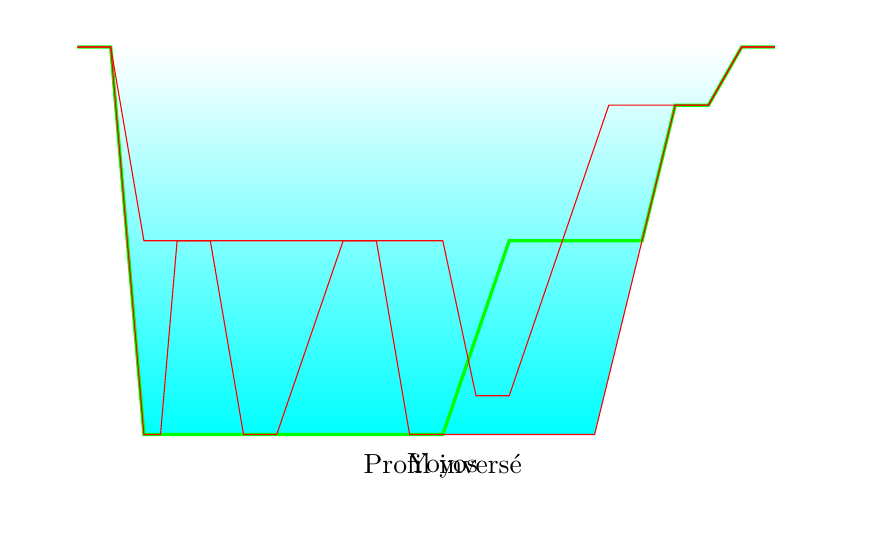
\begin{tikzpicture}[y=-7pt,x=12pt]
\path[use as bounding box] (-2.5,25) rectangle (22.5,-1);
\shade[top color=white,bottom color=cyan] (0,0) -- (1,20) -- (10,20) -- (14.5714,20) -- (17,3) -- (18,3) -- (19,0);
\draw[green, very thick] (-1,0) -- (0,0) -- (1,20) -- (10,20) -- (12,10) -- (16,10) -- (17,3) -- (18,3) -- (19,0) -- (20,0);
%%% premier profil à risque : yoyos
\draw<2>[red] (-1,0) -- (0,0) -- (1,20) -- (1.5,20) -- (2,10) -- (3,10) -- (4,20) -- (5,20) -- (7,10) -- (10,10) -- (11,18) -- (12,18) -- (15,3) -- (18,3) -- (19,0) -- (20,0);
%\node<2>[xscale=-1,anchor=south,inner sep=0pt] at (-1,0) {\twemoji{woman walking}};
%\node<3> at (0,0)    {\twemoji{mermaid}};
%\node<4> at (1.25,20){\twemoji{mermaid}};
%\node<5> at (2.5,10) {\twemoji{mermaid}};
%\node<6> at (4.5,20) {\twemoji{mermaid}};
%\node<7> at (8.5,10) {\twemoji{mermaid}};
%\node<8> at (11.5,18){\twemoji{mermaid}};
%\node<9> at (16.5,3) {\twemoji{mermaid}};
%\node<10> at (19,0)  {\twemoji{mermaid}};
%\node<11>[xscale=-1,anchor=south,inner sep=0pt] at (20,0) {\twemoji{woman walking}};
%%% deuxième profil à risque : profil inversé
\draw<3>[red] (-1,0) -- (0,0) -- (1,10) -- (8,10) -- (9,20) -- (14.5714,20) -- (17,3) -- (18,3) -- (19,0) -- (20,0);
%\node<12>[xscale=-1,anchor=south,inner sep=0pt] at (-1,0)   {\twemoji{woman walking}};
%\node<13> at (0,0)     {\twemoji{mermaid}};
%\node<14> at (4.5,10)  {\twemoji{mermaid}};
%\node<15> at (11.5,20) {\twemoji{mermaid}};
%\node<16> at (17.5,3)  {\twemoji{mermaid}};
%\node<17> at (19,0)    {\twemoji{mermaid}};
%\node<18>[xscale=-1,anchor=south,inner sep=0pt] at (20,0)   {\twemoji{woman walking}};
%%%%%% sat/desat
%\node<-3,11-13,18>[anchor=south, inner sep=0pt] at (19,20) {\includegraphics[height=3cm]{lungs_sat_00}};
%\node<4,6,8>[anchor=south, inner sep=0pt]       at (19,20) {\includegraphics[height=3cm]{lungs_sat_30}};
%\node<5,7,14>[anchor=south, inner sep=0pt]      at (19,20) {\includegraphics[height=3cm]{lungs_sat_2a}};
%\node<15>[anchor=south, inner sep=0pt]          at (19,20) {\includegraphics[height=3cm]{lungs_sat_32}};
%\node<9-10>[anchor=south, inner sep=0pt]        at (19,20) {\includegraphics[height=3cm]{lungs_sat_1b}};
%\node<16-17>[anchor=south, inner sep=0pt]       at (19,20) {\includegraphics[height=3cm]{lungs_sat_1d}};
%%
\node<2>[anchor=north] at (10,20.5) {Yoyos};
\node<3>[anchor=north]  at (10,20.5) {Profil inversé};
\end{tikzpicture}
\end{frame}

\begin{frame}{\EMPH{LA} méthode 100~\% résultats garantis}
\begin{exampleblock}{\centering Si je ne suis pas sûr(e)}
\centering\rule{0pt}{1cm}\Large
Ne pas plonger permet d'éviter l'accident de façon
certaine!\rule[-1cm]{0pt}{0pt}
\end{exampleblock}
\end{frame}

\subsubsection{Vive la science!}

\begin{frame}{L'état de l'art}
{Divers Alert Network (\chref{https://www.daneurope.org/fr/home}{DAN Europe})}

L'étude de \chref{https://journals.viamedica.pl/international_maritime_health/article/view/108038}{Marroni \& al., 2026}\footnote{Alessandro
Marroni, Jacek Kot, Massimo Pieri, Riccardo Pelliccia, and Costantino Balestra.
Identification of DCS risk factors in recreational diving: multifactorial
model based on the DAN DSL Database 2024. \textit{International Maritime
Health}, 77(1) :1 – 12, 2026. ISSN 2081-3252. doi: 10.5603/imh.108038.} 
est à ce jour la meilleure source sur les ADD en plongée loisir.

C'est une analyse statistiques sur les données DAN jusqu'en 2024 

\begin{block}<visible@2>{}
Elle est criticable, mais donne de nouvelles informations
très pertinentes!
\end{block}

\end{frame}

\begin{frame}{Marroni \& al, 2026}
\centering
ADD dans \numprint[\%]{0.49} des cas, \alert{les procédures ont
toujours été respectées}.
\begin{block}<2-3>{Facteurs favorisant}
\begin{enumerate}
\item Sur-saturation en sortie de plongée (ZH-L16C); \tikz[remember picture]\node[inner xsep=0pt] (zh) {};
\item<alert@3> être une femme; \addtocounter{enumi}{-1}
\item le compartiment directeur en sortie de plongée.\only<3>{\begin{tikzpicture}[overlay,remember picture]\node (s) at (0,0){};\draw[-stealth] (s) to[bend right] (zh);\end{tikzpicture}}
\end{enumerate}
\end{block}

\begin{block}<4->{Facteurs améliorant}
\begin{itemize}
\item Plus de plongées consécutives;
\item plus de fatique ressentie;
\item moins de confort thermique.
\end{itemize}
\end{block}
\visible<5>{\textcolor{example text.fg}{$\Rightarrow$ Comportements adaptés intégrés par les plongeurs et plongeuses}}
\end{frame}

\begin{frame}{Quoi en conclure?}
Gros problèmes d'échantillonnage certes, mais cette étude permet
quelques conclusions.
\begin{exampleblock}{Les \og bons \fg\ comportements}
\begin{itemize}
\item[\ensuremath{\Rightarrow}] Continuer à favoriser les comportements sécuritaires en cas de froid, fatigue, \dots
\item[\ensuremath{\Rightarrow}] Porter plus d'attention aux plongées engagées!
\item[\ensuremath{\Rightarrow}] Paliers profonds dangereux!
\item[\ensuremath{\Rightarrow}] Être plus prudent si on est ou plonge avec une femme.
\end{itemize}
\end{exampleblock}
\end{frame}

\subsection{Ordinateurs \& tables}

\subsubsection{Les tables MN90}

\input{common/table}

\subsubsection{Les ordinateurs}

\begin{frame}{Un ordinateur de plongée}
\begin{itemize}
\item Peut toujours calculer MAIS pas plus de deux plongées par
  \numprint{24}~heures;
\item vitesse de remontée $\sim\numprint[m\cdot min^{-1}]{10}$, \numprint[m\cdot min^{-1}]{6}
  entre les paliers.
\end{itemize}
\end{frame}

\begin{frame}{Affichage}
\centering
\includegraphics<1>[width=10cm]{ordinateur-de-plongee}\\
source image: \chref{https://differentdive.com/ordinateur-de-plongee/}{differentdive.com}
\end{frame}

\begin{frame}{Un ordinateur de plongée}{\only<-5>{Savoir le lire}\only<6->{Savoir l'utiliser}}
\centering
\includegraphics<-5>[width=5cm]{suunto}%
\only<-5>{\\Suunto%
\begin{tikzpicture}[overlay,remember picture, every pin edge/.style={stealth-,shorten <=2pt, green!60!black,thick}]
\node<2->[draw,green,thick,shape=ellipse,pin={[pin distance=1cm]30:Profondeur}] at (-0.4,4.6) {\rule{1cm}{0pt}\rule{0pt}{5mm}};
\node<3->[draw,green,thick,shape=ellipse,pin={[pin distance=8mm]right:Temps de plongée}] at (0.3,3.5) {\rule{1cm}{0pt}\rule{0pt}{5mm}};
\node<4->[draw,green,thick,shape=ellipse,pin={[pin distance=1.2cm,text width=3cm,align=right]left:Temps avant palier/paliers}] at (-1.25,3.5) {\rule{5mm}{0pt}\rule{0pt}{5mm}};
\node<5>[text width=3cm] at (-4,5) {Profondeur max, vitesse de remontée, \dots};
\end{tikzpicture}}%
\begin{columns}<only@6->[c]
\begin{column}{0.32\textwidth}
\begin{itemize}[<+(5)->]
\item Date \& heure
\item Planification
\item Mélange gaz
\item Durcir
\item Log
\end{itemize}
\end{column}
\begin{column}{0.6\textwidth}
\raggedleft

\includegraphics[width=\textwidth]{manual}\\[-10pt]
\scriptsize pch.vector (Magnific)
\end{column}
\end{columns}
\end{frame}

\subsubsection{Facteur de gradient}

\begin{frame}{Un peu de contexte}
\centering
\begin{tikzpicture}
\pgfmathparse{1.1696 + 7/0.5578}\let\bul\pgfmathresult
\pgfmathparse{1.1696 + 1/0.5578}\let\bulh\pgfmathresult
\begin{axis}[clip=false,
  axis lines=left, axis on top,
	ymin=0,
	xmin=0,
  xtick={0}, xticklabels={Surface},
  ytick=\empty,
  xticklabel style={font=\tiny},
  xlabel={Profondeur}, ylabel={$P_{\text{compart}}$},
  domain=0:60, name=desat
]
\fill<6>[blue!10] (0,1) -- (60,7) -- (60,1) -- cycle;
\fill<7>[blue!10] (0,1) -- (60,7) -- (60,\bul) -- (0,\bulh) -- cycle;
\fill<8>[blue!10] (0,\bulh) -- (60,\bul) -- (desat.north east) -- (desat.north west) -- cycle;
\addplot[] {1 + x/10};
\addplot[teal] {1};
\node[anchor=base west] at (60,7) {$P_\text{ext}$};
\node[anchor=base west] at (60,1) {$P_\text{atm}$};
\addplot[violet, name path=Bulh]{1.1696 + (1 + x/10)/0.5578};
\node[violet,anchor=base west] at (60,\bul) {$P_\text{Bülhman}$};
\only<5>{\addplot[blue,thick] {1 + x/10};}
\node<9->[inner sep=0pt] (mer) at (50,5) {\texttwemoji{merperson}};
\path[name path=mermaid] (0,5) -- (60,5);
\path[name path=sec pal] (0,3.5) -- (60,3.5) -- (60,0) -- (0,0);
%%
\path[name intersections={of=Bulh and mermaid, by={pal}}, name path=fpal] (pal) -- ++(0,-5.2);
\path[name intersections={of=Bulh and sec pal, by={pall}}, name path=spal] (pall) -- ++(0,-3.2);
\path[name path=sortie] (0,2.5) -- (60,2.5);
\path[name path=ftime] (40,5) -- (40,0);
%
\draw<10->[dashed,name intersections={of=Bulh and mermaid, by={first pal}}, name intersections={of=Bulh and sec pal, by={sec}}] (mer) -- (first pal) |- (sec) |- (0,2.5);
\draw<11->[green!60!black,-stealth,name intersections={of=sec pal and fpal, by={a,b}}] (a) -- (b) node[below,font=\scriptsize]{Premier palier};
\draw<12>[green!60!black,dashed,name path=time,name intersections={of=sortie and spal,by={out}}] (out) -- ++(40,0);
\draw<12>[green!60!black,stealth-stealth,name intersections={of=time and ftime,by={a}},name intersections={of=ftime and mermaid,by={b}}] (a) -- (b) node[right,pos=0.5,font=\scriptsize]{Temps total de palier};
\end{axis}
\node<2-5>[inner sep=0pt,anchor=north west] (comp) at (desat.above north west) {\includegraphics[width=2cm]{desat_eq}};
\node<6>[inner sep=0pt,anchor=north west] (comp) at (desat.above north west) {\includegraphics[width=2cm]{desat_air}};
\node<7>[inner sep=0pt,anchor=north west] (comp) at (desat.above north west) {\includegraphics[width=2cm]{desat_liq}};
\node<8>[inner sep=0pt,anchor=north west] (comp) at (desat.above north west) {\includegraphics[width=2cm]{desat_bulle}};
\draw<3>[blue,thick,-stealth] (0,0) -- (desat.north west);
\draw<4>[blue,thick,-stealth] (0,0) -- (desat.south east);
\begin{pgfonlayer}{background}
\fill<3>[blue!10] (comp.west) rectangle ([yshift=-3pt]comp.south east);
\fill<4>[blue!10] (comp.west) rectangle (comp.north east);
\end{pgfonlayer}
%%
\end{tikzpicture}
\end{frame}

%\input{common/facteur_gradient}
\input{common/facteur_gradient_graphics}
